\documentclass[manuscript,nonacm]{acmart}

% ============================================================
% Predicting Albanian Student Low-Proficiency Risk from OECD PISA (2009-2022)
% Conference-style manuscript (EDM / LAK register), ACM sigconf layout.
% nonacm: drop ACM copyright/DOI apparatus for a course/preprint build.
% ============================================================

\settopmatter{printacmref=false}
\renewcommand\footnotetextcopyrightpermission[1]{}
\pagestyle{plain}

\usepackage{booktabs}
\usepackage{graphicx}
\usepackage{subcaption}

\graphicspath{{figures/}}

\begin{document}

\title{A Structural Break, Not a Weaker Cohort: Explaining Albania's 2022
PISA Collapse with Survey-Weighted Machine Learning}

\author{Xhoi Ikonomi}
\affiliation{%
  \institution{Metropolitan University of Tirana}
  \department{MSc Artificial Intelligence (Data Science profile)}
  \city{Tirana}
  \country{Albania}
}
\email{ikonomixhoja@gmail.com}

\begin{abstract}
Albania's share of 15-year-olds below PISA mathematics Level~2 rose from 42\% in
2018 to 75\% in 2022, the sharpest regression in the assessment. We ask whether
machine learning on background questionnaire data can identify at-risk students,
\emph{why} they are at risk, and whether the 2022 collapse is merely a lower-scoring
cohort or a change in the risk structure itself. Using all five Albanian PISA cycles
(2009--2022; 27{,}042 students) and eight comparison countries (323{,}121 students),
and applying the survey methodology PISA requires, final student weights on every
estimate, plausible values combined by Rubin's rules, and balanced repeated
replication for design-based standard errors, we report four findings. First, a
domain classifier separates 2018 from 2022 Albanian students with AUC~0.98 on
background features alone: the collapse is a \emph{structural covariate shift}, not
just lower scores. Second, individual background variables hit an accuracy ceiling
(weighted cross-validated AUC~0.73) that hyperparameter tuning cannot move, but adding
survey-weighted \emph{school socioeconomic composition} lifts every model by
$\sim$0.05 AUC to $\sim$0.78 and makes gradient boosters significantly outperform
logistic regression. Third, that $\sim$0.78 is a genuine data ceiling: a multilevel
model (school ICC~$\approx$~0.31) and a direct school-questionnaire linkage
(no significant gain, all $p>0.24$) independently converge on it. Fourth, the crisis
is \emph{broad-based}: Albania has the flattest SES gradient of the nine countries, its
risk drivers (math anxiety, school composition) are shared with peers, and a fairness
audit shows a naive threshold over-flags the poorest quintile. We release a calibrated,
interpretable risk screener but frame it as associational, not a policy lever.
\end{abstract}

\keywords{PISA, educational data mining, covariate shift, survey weights,
plausible values, model calibration, algorithmic fairness, low proficiency}

% acmart's manuscript byline sets the author line in ALL CAPS via \MakeUppercase.
% Neutralise it just around \maketitle (page style is plain, so no header/other
% caps are affected) so the byline reads in normal case.
\makeatletter
\let\ORI@MakeUppercase\MakeUppercase
\renewcommand{\MakeUppercase}[1]{#1}
\makeatother
\maketitle
\makeatletter
\let\MakeUppercase\ORI@MakeUppercase
\makeatother

\section{Introduction}

In four years, three in four Albanian fifteen-year-olds crossed the line into low
mathematics proficiency. The OECD Programme for International Student Assessment
(PISA) measures whether students can apply reading, mathematics, and science to real
problems, and its \emph{Level~2} boundary marks basic proficiency; students below it
are the international ``low performers'' that education systems target. In PISA~2018,
42\% of Albanian students fell below the mathematics Level~2 line. In PISA~2022, 75\%
did. No other participating system regressed so far in a single cycle. A drop of this
magnitude invites an obvious reading: the 2022 cohort was simply weaker, and the
country needs broad remediation. Whether that reading is right is not a semantic
question. It determines whether policy should treat 2022 as more of the same, only
worse, or as evidence that \emph{who} is at risk, and \emph{why}, has changed.

This paper treats the question as one of educational data mining, and it insists on
the survey methodology that PISA requires. PISA is a stratified, clustered sample
reported through final student weights, and each achievement score arrives as ten
\emph{plausible values}, multiple imputations of a latent proficiency. Analyses that
ignore the weights do not estimate a population quantity, and analyses that collapse
the plausible values to a single number understate their uncertainty. A large body of
secondary PISA work nonetheless does both. Every estimate below is survey-weighted;
plausible values are combined by Rubin's rules; and where the data permit (the
2015, 2018, and 2022 cycles carry 80 balanced-repeated-replication weights) standard
errors are design-based.

From the student background questionnaire, socioeconomic status, home possessions,
parental education and occupation, grade repetition, immigration status, school
belonging, teacher support, math anxiety, and access to information technology, we ask
three questions. Can a classifier identify Albanian students at risk of low
mathematics proficiency, and how well? Which factors drive that risk, and do they
differ from the drivers in comparable countries? And does the 2022 collapse represent
a change in the risk \emph{structure} that can explain the 2018-to-2022 reversal? The
economic and structural conditions of Albania in this exact window, a destructive 2019
earthquake, an extended pandemic school closure, a thin remote-learning infrastructure,
and sustained emigration of working-age adults and teachers, give these questions a
concrete backdrop that we return to in Section~\ref{sec:context}.

\paragraph{Thesis.}
Albania's 2022 mathematics collapse is not a uniformly weaker cohort but a
\emph{structural break in the risk-generating process}, driven by a disruption to the
supply of schooling rather than to household resources; the students at risk are
identifiable from background data only up to a genuine ceiling of about 0.78 AUC that
three independent methods confirm, their risk is broad-based rather than concentrated
in the poor, and its drivers are the same ones that operate across the region.

\paragraph{Roadmap.}
Section~\ref{sec:data} describes the five-cycle data and the design-based estimation.
Section~\ref{sec:methods} sets out the leakage-safe, survey-weighted modelling and the
covariate-shift diagnostic. Section~\ref{sec:results} reports the four empirical
findings: the structural shift (AUC~0.98), the feature-versus-data ceiling, the shared
and broad-based driver structure, and the calibrated, fairness-audited screener.
Section~\ref{sec:context} then reads those findings against Albania's economic and
structural conditions, arguing that a supply-side shock, not a household-income shock,
best fits the evidence. Section~\ref{sec:discussion} discusses implications and limits,
and Section~\ref{sec:conclusion} returns to the collapse with which we began.

\paragraph{Contributions.}
Our central contribution is methodological and, we believe, transferable beyond this
dataset: we show that the accuracy ceiling recurring across PISA prediction studies is
not one phenomenon but two, a movable \emph{feature} ceiling and a fixed \emph{data}
ceiling, and that the two can be told apart with convergent evidence rather than with
another round of tuning. Applied to Albania, this lets us (i) show the 2022 collapse is
a structural covariate shift rather than a level change; (ii) locate the background-data
accuracy ceiling, demonstrate it is a feature ceiling by moving it with school
socioeconomic composition, and then certify the new plateau as a genuine data ceiling
through three independent routes; (iii) characterise the crisis as broad-based and
shared with regional peers; and (iv) connect these statistical findings to Albania's
economic and structural context, while delivering a calibrated, interpretable, and
honestly-bounded risk screener that we argue should not be read causally.

\section{Background and Related Work}

\paragraph{PISA methodology.}
PISA reports each student's proficiency as ten plausible values drawn from a
posterior latent-trait distribution, and every published statistic is weighted by
the final student weight with variance estimated by balanced repeated replication
(BRR)~\cite{oecd2024pisa,oecd2009manual}. Rubin's rules combine point estimates and
between-imputation variance across the plausible values~\cite{rubin1987}. These are
not optional refinements: using a single averaged score as a target understates
uncertainty, and unweighted statistics do not estimate a population quantity. Much
secondary PISA analysis nonetheless drops both. We follow the manual throughout.

\paragraph{Machine learning on PISA.}
A body of work predicts proficiency or at-risk status from PISA background data with
tree ensembles and reports feature importances (e.g.\ socioeconomic status, grade
repetition, and school climate as recurring drivers). Gradient-boosted trees,
XGBoost~\cite{chen2016xgboost}, LightGBM~\cite{ke2017lightgbm}, and
CatBoost~\cite{prokhorenkova2018catboost}, are the usual strong baselines on this
tabular regime, and SHAP values~\cite{lundberg2017shap} the usual explanation. Our
contribution is less a new model than a methodologically disciplined one: weighted
throughout, leakage-controlled, with model differences tested rather than ranked.

\paragraph{Dataset shift.}
When the input distribution changes between two populations, a classifier trained to
tell them apart quantifies the shift; a high domain-classifier
AUC is direct evidence of covariate shift~\cite{quinonero2009dataset}. We use this
as the central diagnostic for the 2018$\rightarrow$2022 change rather than only
comparing marginal score distributions.

\paragraph{Calibration, decision curves, and fairness.}
A screening probability must be calibrated to be actionable; isotonic
regression is a standard non-parametric post-hoc
calibrator~\cite{zadrozny2002isotonic}, and decision-curve analysis evaluates a
screener by net benefit across operating thresholds rather than by accuracy at a
single cut~\cite{vickers2006dca}, important when prevalence is high. Group-fairness
diagnostics (demographic parity, equalized odds) expose disparate error rates across
protected groups~\cite{hardt2016equalized}. We report all three, survey-weighted.

\paragraph{Nested design and honest comparison.}
PISA students are nested in schools, so a random-intercept (multilevel) logistic
model is the design-appropriate specification and its intraclass correlation
quantifies between-school variance~\cite{goldstein2011multilevel}. Finally, because
repeated cross-validation folds share training data, naive fold-score intervals are
anti-conservative; we use the Nadeau--Bengio corrected-resampled
variance~\cite{nadeau2003inference} and compare models with the corrected resampled
$t$-test (in-sample) and the DeLong test on shared test
predictions~\cite{delong1988}.

\section{Data}
\label{sec:data}

We use the student questionnaire files for all five PISA cycles from 2009 to 2022.
The 2015/2018/2022 cycles ship as SPSS \texttt{.sav}; 2009 and 2012 are fixed-width
ASCII with SPSS control files, which we parse with a purpose-built reader. After
harmonising feature names across cycles, the Albanian longitudinal file holds
27{,}042 students; a comparison set of nine countries, Albania, North Macedonia,
Montenegro, Serbia, Bulgaria (Balkan peers), Estonia and Finland (top performers),
and Mexico and Colombia (GDP-matched), holds 323{,}121 students. Raw files are
multi-gigabyte and not redistributed; processed slices are regenerated by the
pipeline.

\paragraph{Target.}
A student is \emph{at risk} if their mathematics score falls below the exact OECD
Level~2 boundary of 420.07 points. Because each score is ten plausible values, the
model-comparison target is the point (PV-mean) indicator, while the final estimates
use per-plausible-value targets combined by Rubin's rules.

\paragraph{Features.}
The core set is thirteen background variables with high cross-cycle availability:
ESCS (the OECD socioeconomic index), home possessions, parental education (HISCED)
and occupation (HISEI), gender, grade repetition, immigration status, school
belonging, teacher support in mathematics, math anxiety, grade relative to modal, and
home/school ICT resources. Composite and interaction features (a standardised SES
composite, a material-deficit rank, digital-readiness indices, and centred
interaction terms) are derived \emph{inside} the cross-validation pipeline on the
training fold only, so their scaling and rank statistics never leak from the test
fold.

\paragraph{Design-based estimates.}
The 2015/2018/2022 cycles carry 80 Fay balanced-repeated-replication weights; we
combine the BRR sampling variance with the between-plausible-value variance to report
the standard error the OECD manual prescribes. The 2009/2012 fixed-width cycles do
not carry replicate weights and fall back to an imputation-only standard error, which
we flag. Table~\ref{tab:trajectory} gives Albania's weighted at-risk trajectory with
these design-based standard errors: a V-shape that falls from 68\% (2009) to 42\%
(2018) and then snaps back to 74\% in 2022 (Figure~\ref{fig:trajectory}).

\begin{table}[t]
\centering
\caption{Albania weighted at-risk mathematics rate (below Level~2) with
design-based standard errors. BRR available only for the SPSS cycles.}
\label{tab:trajectory}
\begin{tabular}{lcccc}
\toprule
Cycle & At-risk & SE & 95\% CI & BRR \\
\midrule
2009 & 0.677 & 0.0076 & 0.663--0.692 & n/a \\
2012 & 0.607 & 0.0051 & 0.597--0.617 & n/a \\
2015 & 0.533 & 0.0108 & 0.512--0.554 & \checkmark \\
2018 & 0.424 & 0.0088 & 0.407--0.441 & \checkmark \\
\textbf{2022} & \textbf{0.739} & \textbf{0.0041} & \textbf{0.731--0.747} & \checkmark \\
\bottomrule
\end{tabular}
\end{table}

\begin{figure}[t]
\centering
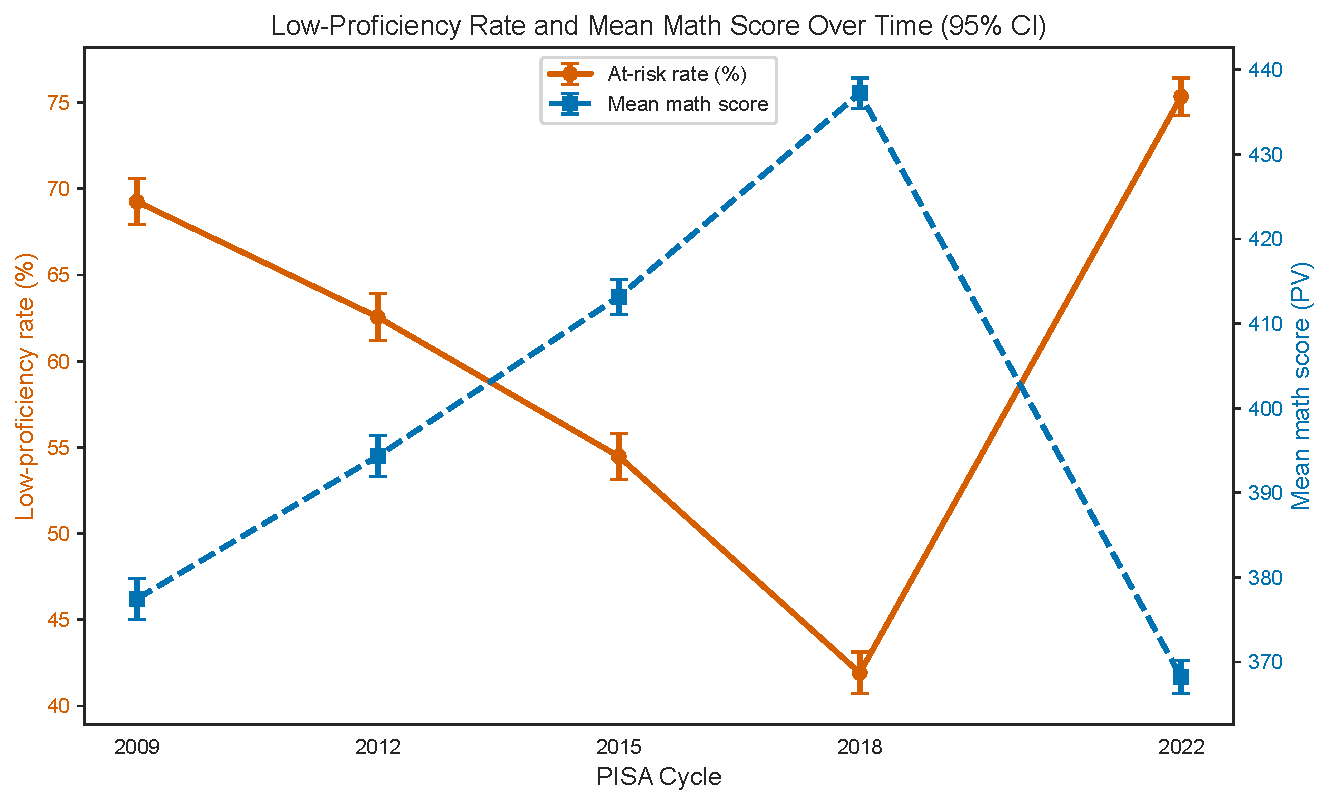
\includegraphics[width=0.8\linewidth,height=0.33\textheight,keepaspectratio]{A1_atrisk_trajectory}
\caption{Albania's weighted below-Level-2 mathematics rate, 2009--2022. The 2018 low
(42\%) and the 2022 spike (74\%) bracket the structural break this paper explains.}
\label{fig:trajectory}
\end{figure}

\paragraph{A verified data gap.}
Albania genuinely lacks the ESCS index in 2012 and 2015 (an OECD coverage gap
confirmed against the source files, not a processing bug), whereas all peer countries
have full 2015 background data. This limits Albania's \emph{own} cross-cycle
socioeconomic comparison but leaves the 2018-vs-2022 shift analysis, both cycles
fully covered, unaffected.

\section{Methods}
\label{sec:methods}

\subsection{Survey-correct estimation}
Every descriptive statistic and every model metric is weighted by the final student
weight $W_{\mathrm{FSTUWT}}$. Where a model is fit, weights are routed to the
estimator's own \texttt{sample\_weight} (correcting a subtle bug in which
scaler-wrapped models, logistic regression, SVM, KNN, MLP, silently fell back
to an unweighted fit because the weight was passed to the wrong pipeline step).
Class-conditional statistics rescale the population-scale weights to the effective
sample size before, e.g., a $\chi^2$ test, so significance is not inflated by the
weight magnitudes.

\subsection{Leakage-safe pipeline}
Each fold's pipeline is: (1) an engineered-feature builder that learns component
means, standard deviations, and the home-possessions rank curve on the training fold
and replays them on the test fold; (2) median imputation fit on the training fold;
(3) the estimator. Interaction terms are built from mean-centred components so a
product is not confounded with its main effects. School-composition features are
survey-weighted, \emph{leave-one-out} school means (a student's own value is excluded
from their school mean), and a fold-safe re-computation that recomputes the means
from the training fold only reproduces an identical effect, so the lift is
compositional, not leakage.

\subsection{Evaluation and comparison}
Models are scored with repeated stratified $5\times4$ cross-validation, weighted ROC
and PR AUC, F1-macro, and MCC. Fold-score confidence intervals use the
Nadeau--Bengio corrected-resampled variance, which replaces the naive $1/k$ term with
$1/k + n_{\text{test}}/n_{\text{train}}$ to account for the correlation between folds
that share training data. Model-vs-model differences are tested directly: the
corrected resampled $t$-test on paired per-fold AUCs (cross-validation) and the
DeLong test on shared test-set predictions (out-of-sample). This turns a ranking
table into a claim about which gaps are real.

\subsection{Covariate-shift diagnostic}
To quantify the 2018$\rightarrow$2022 change we train a domain classifier to
distinguish the two cohorts from background features alone, with weighted subsampling,
pooled-median imputation, and missingness indicators; a high AUC certifies that the
input distribution, not just the score level, moved. We validate the diagnostic
on a null (same cohort split at random $\rightarrow$ AUC~$\approx$~0.5).

\subsection{Explanation, calibration, fairness, forecast}
We compute TreeSHAP global and per-student attributions on the school-context model,
and partial-dependence / centred-ICE curves for the top drivers. For deployment we
add out-of-fold isotonic calibration and tune the decision threshold on calibrated
out-of-fold predictions to maximise weighted MCC. The fairness audit reports weighted
demographic parity, equal-opportunity (TPR) and false-positive-rate gaps across
gender, SES quintile, and immigration status, plus a threshold sweep. A random-intercept
logistic model provides the design-appropriate specification and the between-school
intraclass correlation. Finally, a scenario Monte-Carlo forecast for 2026 propagates
each cycle's design-based standard error through a weighted trend fit; with only five
cycles and a structural break we report scenarios and their intervals, not a point
prediction.

\subsection{Robustness and extension analyses}
Five further analyses probe the main claims. (i) \emph{Cross-country ceiling
replication}: the student-only versus school-context comparison is re-run identically in
all nine systems, and each system's between-school ICC is read from its random-intercept
model, to test whether the feature ceiling and its size generalise. (ii) \emph{Modality
ablation}: PISA's computer-based cognitive-process indicators are added to the
school-context model and split into cognitive-process and questionnaire-process blocks,
so an endogenous within-test signal can be separated from data available at screening
time. (iii) \emph{Fairness mitigation}: group-specific decision thresholds are fit on
calibrated out-of-fold scores to equalise the per-quintile false-positive rate
(equalized-odds post-processing), tracing the accuracy--equity frontier. (iv)
\emph{Partial identification}: given the 79\% coverage index, worst-case and monotone
Manski bounds on the population at-risk rate are computed, the monotone bound assuming
the out-of-frame group is no better off than the assessed. (v) \emph{Difference-in-differences}:
a design-based DiD contrasts the earthquake-affected central region with the rest of the
country across 2018 and 2022, with a 2015$\rightarrow$2018 placebo to test parallel
trends; weights, plausible values, and replicate-weight standard errors are carried
throughout.

\subsection{Reproducibility and engineering}
Logic lives in unit-tested modules (177 tests on synthetic fixtures, covering the
weighted statistics, Rubin's rules, the leakage-safe transformer, the BRR+PV variance,
the Manski bounds and group-threshold mitigation, and the Nadeau--Bengio / DeLong
maths); notebooks are narrative layers over them. On
macOS the boosters (Homebrew \texttt{libomp}) and scikit-learn (bundled OpenMP) can
abort a process if their runtimes collide; we isolate each model fit in a fresh
subprocess that imports the boosters before scikit-learn, which resolved an
import-order segfault and returned LightGBM to the comparison.

\section{Results}
\label{sec:results}

\subsection{The 2022 collapse is a structural shift}
A domain classifier separates 2018 from 2022 Albanian students with weighted
AUC~\textbf{0.98} on background features alone. The 2022 cohort is not simply a
lower-scoring version of 2018 along a stable structure; the input distribution
itself moved. The most-shifted variables (Figure~\ref{fig:drift}) are teacher support
in mathematics (standardised mean difference $-0.31$) and home possessions ($+0.27$),
with school belonging, grade repetition, and ESCS following. That teacher support
fell while reported home possessions rose is consistent with a disruption to the
\emph{schooling process} rather than a household-wealth shock, and it foreshadows the
compositional result below. Out-of-sample the shift is detectable but not
catastrophic: models trained on 2009--2018 still transfer to 2022 at AUC~$\approx$~0.67
(covariate shift without total collapse).

\begin{figure}[t]
\centering
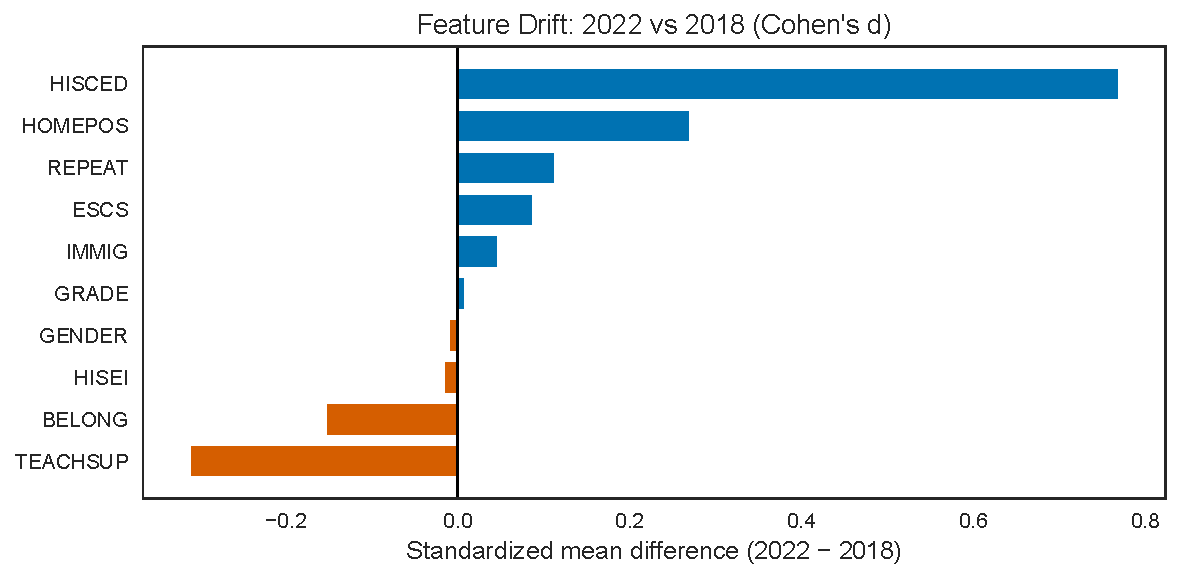
\includegraphics[width=0.8\linewidth,height=0.33\textheight,keepaspectratio]{B5_feature_drift}
\caption{Standardised 2018$\rightarrow$2022 drift of Albanian background features.
Teacher support and home possessions move most; the domain classifier that
separates the cohorts reaches AUC~0.98.}
\label{fig:drift}
\end{figure}

\subsection{An accuracy ceiling, and its cause}
On the thirteen student features, twelve estimators cluster tightly
(Figure~\ref{fig:models}). CatBoost leads at weighted CV AUC~0.731, but a paired
Nadeau--Bengio test finds the top three statistically \emph{tied}: CatBoost
$\approx$ logistic regression ($p=0.50$) $\approx$ gradient boosting ($p=0.37$): a
transparent linear model matches the best boosters. Nested-CV Optuna tuning of the
top three yields no significant gain (CatBoost $+0.002$, $p=0.81$; GBM $+0.004$,
$p=0.45$; LR $-0.001$, $p=0.43$). This looks like a data ceiling.

It is not; it is a \emph{feature} ceiling. Adding survey-weighted, leave-one-out
\textbf{school-mean} ESCS, home possessions, anxiety, and teacher support, plus cohort size,
lifts every model by $\sim$0.05 AUC (Table~\ref{tab:models}): CatBoost
$0.731\rightarrow\mathbf{0.783}$, and the effect is identical under fold-safe
re-computation. Crucially, adding school context \emph{breaks the tie}: the boosters
now beat logistic regression significantly (GBM vs LR $p=0.001$), because they exploit
a student $\times$ school-composition interaction a linear model cannot. SVM and MLP,
added for completeness, land mid-table: the podium is a booster story, not an
artefact of omitting kernel or neural learners.

\begin{table}[t]
\centering
\caption{Albania 2022, weighted $5\times4$ CV, \emph{with} school context.
$\Delta$AUC is the lift over the student-only baseline.}
\label{tab:models}
\begin{tabular}{lccccc}
\toprule
Model & AUC & $\Delta$AUC & PR-AUC & F1 & MCC \\
\midrule
\textbf{CatBoost}   & \textbf{0.783} & $+0.052$ & 0.907 & 0.693 & 0.393 \\
Gradient Boosting   & 0.777 & $+0.050$ & 0.905 & 0.665 & 0.365 \\
LightGBM            & 0.775 & $+0.060$ & 0.902 & 0.688 & 0.381 \\
Random Forest       & 0.769 & $+0.060$ & 0.895 & 0.644 & 0.345 \\
Extra Trees         & 0.758 & $+0.051$ & 0.884 & 0.641 & 0.332 \\
XGBoost             & 0.756 & $+0.058$ & 0.892 & 0.657 & 0.333 \\
Logistic Regression & 0.754 & $+0.027$ & 0.897 & 0.649 & 0.332 \\
SVM (RBF)           & 0.749 & $+0.037$ & 0.894 & 0.609 & 0.282 \\
MLP (128-64)        & 0.743 & $+0.034$ & 0.884 & 0.620 & 0.295 \\
Naive Bayes         & 0.701 & $+0.019$ & 0.856 & 0.610 & 0.263 \\
KNN                 & 0.700 & $+0.036$ & 0.861 & 0.613 & 0.257 \\
Decision Tree       & 0.609 & $+0.041$ & 0.797 & 0.608 & 0.217 \\
\bottomrule
\end{tabular}
\end{table}

\begin{figure}[t]
\centering

\includegraphics[width=0.8\linewidth,height=0.33\textheight,keepaspectratio]{C4_model_comparison_auc}
\caption{Weighted CV AUC with Nadeau--Bengio intervals. Boosters form a top band once
school context is included; the interpretable logistic-regression baseline gains least
because it cannot use the student $\times$ school interaction.}
\label{fig:models}
\end{figure}

\subsection{$\sim$0.78 is a genuine data ceiling}
Three independent routes converge on $\sim$0.78. (i) The composition booster above
plateaus there. (ii) A random-intercept logistic model, the design-appropriate
specification, \emph{matches} the hand-crafted school-mean booster on identical
folds (CV AUC~$\approx$~0.78) and reports a school intraclass correlation
ICC~$\approx$~0.31: about a third of risk variance is \emph{between} schools and
barely touched by student features. (iii) Linking the PISA school questionnaire
(principal-reported resources, staff, class size, leadership) directly onto students
adds no significant signal beyond composition (best $+0.004$ AUC, all $p>0.24$),
because school-mean SES already proxies the school inputs. The ceiling is a property
of what background questionnaires can measure, not of tuning or model capacity. An
ensemble stack of the four boosters confirms this: it reaches AUC~0.786 vs single
CatBoost 0.783 ($+0.003$, $p=0.03$): statistically significant, practically nil,
and it \emph{regresses} MCC and F1 at $\sim$19$\times$ the compute. Single CatBoost
stays the deployable headline.

\subsection{Drivers: anxiety and school composition, shared with peers}
On the school-context model, four of the top seven SHAP drivers are school-level
(Figure~\ref{fig:shap}): school-mean home possessions leads, followed by individual
math anxiety, school-mean teacher support, and school-mean ESCS. The model reads a
student's risk more from the socioeconomic \emph{composition} of their school than
from their own resources; this is the compositional effect made explicit. Immigration
status is negligible. A feature $\times$ country SHAP rank matrix
(Figure~\ref{fig:rankmatrix}) shows these drivers are \emph{shared}: math anxiety is a
top-3 driver almost everywhere (including Estonia), and school composition dominates
most systems. What is distinctive about Albania is the \emph{level and breadth} of low
proficiency, not the mechanism.

\begin{figure}[t]
\centering

\includegraphics[width=0.8\linewidth,height=0.33\textheight,keepaspectratio]{D2_shap_global_bar}
\caption{Global SHAP importance (school-context model). Four of the top seven drivers
are school-level; math anxiety is the strongest individual factor.}
\label{fig:shap}
\end{figure}

\begin{figure}[t]
\centering

\includegraphics[width=0.8\linewidth,height=0.33\textheight,keepaspectratio]{F1_shap_rank_matrix}
\caption{SHAP driver ranks by country. Math anxiety and school composition recur
across systems; Albania mirrors its peers in mechanism.}
\label{fig:rankmatrix}
\end{figure}

\subsection{A broad-based, flat-gradient crisis}
Per-country school-context models (Figure~\ref{fig:gradient}) place Albania at the
highest at-risk rate (75\%) but one of the \emph{lowest} model AUCs (0.77): with three
in four students at risk there is little contrast to separate. Albania also has the
\textbf{flattest} SES gradient of the nine countries ($\sim$17 score points per SD),
a floor effect: even advantaged Albanian students score near 369, close to the
line. Estonia and Finland have \emph{steeper} gradients ($\sim$38--40) yet far higher
levels, because there is more score range for SES to predict. The policy reading is
direct: a flat gradient plus school-composition dominance means SES-targeted transfers
alone miss most at-risk Albanian students; system-wide levers (teacher support,
math-anxiety reduction, raising the floor across all schools) are required.

\begin{figure}[t]
\centering
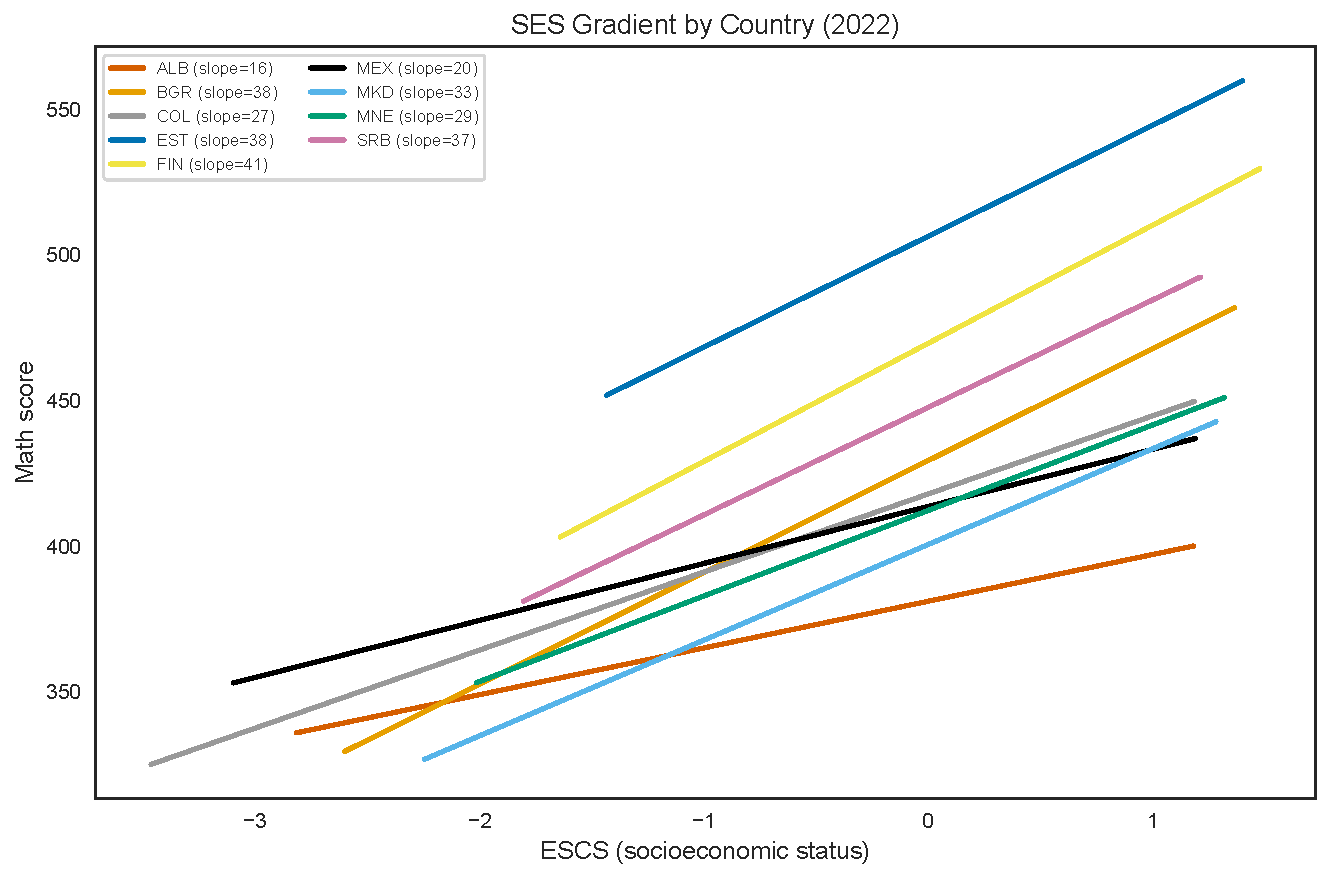
\includegraphics[width=0.8\linewidth,height=0.33\textheight,keepaspectratio]{G2_ses_gradient_2022}
\caption{SES gradient of mathematics score, 2022. Albania's slope is the flattest of
the nine countries, a floor effect, not a steep advantage gap.}
\label{fig:gradient}
\end{figure}

\subsection{A calibrated, fair-audited screener}
Raw CatBoost probabilities are sharp but mis-calibrated (weighted ECE~$\approx$~0.12);
out-of-fold isotonic calibration cuts this to $\approx$~0.01
(Figure~\ref{fig:calibration}), and decision-curve analysis shows the model beats
screen-everyone / screen-no-one across the selective threshold band, the relevant
test at 75\% prevalence. The fairness audit is less comfortable
(Figure~\ref{fig:fairness}): at a fixed threshold the screener over-flags the poorest
SES quintile (false-positive rate $\approx$~0.86 vs $\approx$~0.24 for the richest;
parity gap 0.48, FPR gap 0.63). Because school-mean SES \emph{is} SES, making it a top
feature doubly encodes the gradient; adding school context shrinks the gender gap but
leaves the SES gap intact. This is an equalized-odds concern, and it is why we frame
the screener as a tool to \emph{widen} support, never to ration it.

\begin{figure}[t]
\centering
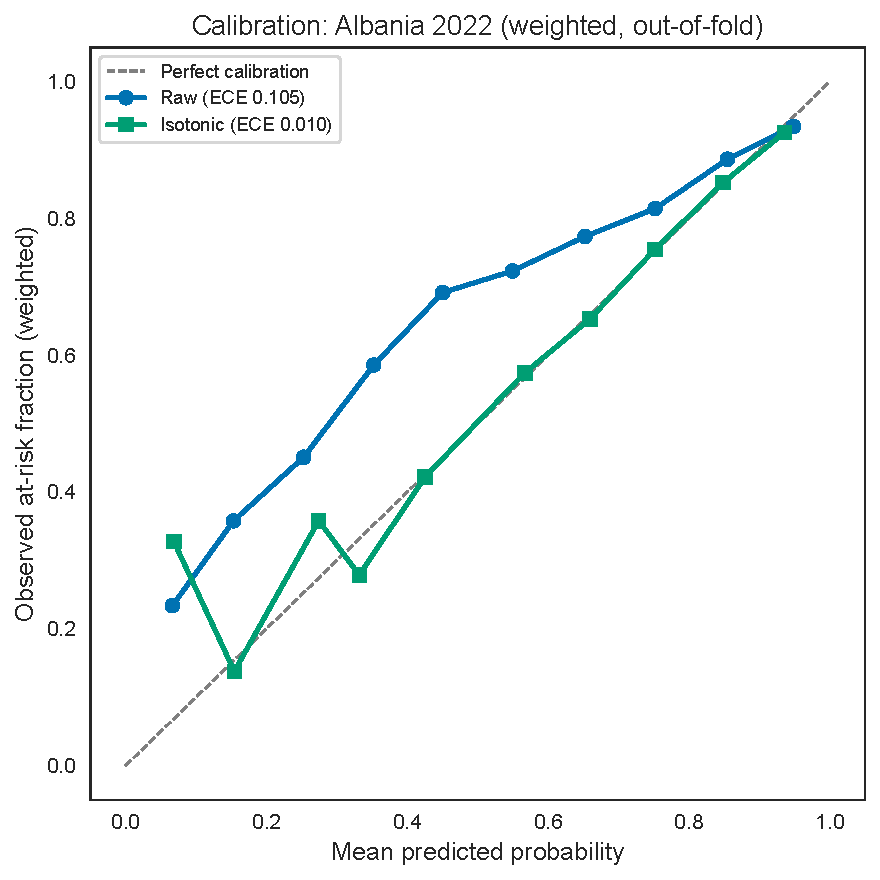
\includegraphics[width=0.8\linewidth,height=0.33\textheight,keepaspectratio]{calibration}
\caption{Reliability curve before/after out-of-fold isotonic calibration; weighted
ECE falls from $\approx$~0.12 to $\approx$~0.01.}
\label{fig:calibration}
\end{figure}

\begin{figure}[t]
\centering

\includegraphics[width=0.8\linewidth,height=0.33\textheight,keepaspectratio]{E1_fairness_threshold_sweep}
\caption{Weighted fairness gaps by decision threshold (gender shown). Gaps shift with
the operating point rather than vanishing, mitigation needs constraints, not a knob.}
\label{fig:fairness}
\end{figure}

\subsection{Forecast for 2026}
With five cycles and a 2022 structural break, a point forecast is indefensible, so we
report scenarios with design-based intervals (Table~\ref{tab:forecast}). The honest
message is the width: absent a strong targeted recovery, the defensible zone runs from
partial reversion ($\sim$47\%) to persistence ($\sim$74\%), both well above Albania's
2018 low of 42\%.

\begin{table}[t]
\centering
\caption{Scenario forecast for the 2026 below-Level-2 rate (Monte-Carlo, design-based
SEs propagated).}
\label{tab:forecast}
\begin{tabular}{lcc}
\toprule
Scenario & 2026 median & 90\% PI \\
\midrule
Persistence (crisis holds)      & \textbf{0.74} & 0.66--0.82 \\
Partial reversion               & 0.47 & 0.43--0.52 \\
Pre-COVID recovery              & 0.21 & 0.18--0.24 \\
\bottomrule
\end{tabular}
\end{table}

\section{The Economic and Structural Context of the Collapse}
\label{sec:context}

The statistical results locate the collapse in time and shape but not in cause; the
economic and structural history of Albania between the 2018 and 2022 assessments
supplies the missing narrative. PISA~2018 was fielded in early 2018 and PISA~2022 in
2022, so any explanation must point to forces that acted in that four-year window. Two
shocks did, and only one of them was shared with Albania's peers.

\paragraph{Two compounding shocks hit the schooling window.}
Albania entered the pandemic already weakened by a natural disaster that its comparison
countries did not face. On 26 November 2019 a magnitude~6.4 earthquake struck the
Durr\"es and Tirana region, the strongest to hit the country in more than four decades;
it killed 51 people, injured about 3{,}000, and damaged or destroyed housing and
schools across roughly a dozen cities in the most populous part of
Albania~\cite{albania_pdna2020}. Barely three months later, COVID-19 closed schools
nationwide from March~2020, and Albania recorded one of the longer cumulative closure
durations in the region before instruction fully
resumed~\cite{unesco2022closures,worldbank_covid_learning}. The comparison economies in
this study lived through the pandemic, but none of them absorbed a major earthquake in
the same window. Notably, the OECD's own country note attributes Albania's 2022 decline
to exactly this pairing, an end-of-2019 earthquake that damaged schools and houses
across twelve cities, compounded by the pandemic~\cite{oecd_albania_note2023}. Albania
therefore experienced a \emph{double} disruption to the continuity of schooling
precisely between the two assessments, which is where a structural break would have to
originate.

\paragraph{The shock was to schooling, not to household wealth, and the data show it.}
If the 2022 collapse were a household-income shock, the socioeconomic markers in the
questionnaire would have fallen; instead, the school-side marker fell while the
household marker held. The covariate-shift analysis (Section~\ref{sec:results}) found
that the variable which moved most from 2018 to 2022 was teacher support in
mathematics, down by roughly a third of a standard deviation, while reported home
possessions actually rose. A demand-side poverty shock would depress home possessions;
the observed pattern instead points to a supply-side degradation of instruction, the
signature of closed and damaged schools and of teaching capacity stretched thin. This
interpretation is consistent with the macroeconomic record: Albania's economy
contracted in 2020 and rebounded strongly the next year, with World Bank figures
placing the contraction at roughly three to four percent and 2021 growth near nine
percent as tourism recovered~\cite{worldbank_albania}, while household consumption was
cushioned throughout by diaspora remittances worth about nine percent of
GDP~\cite{worldbank_remittances}. Family assets did not crater, which is why home
possessions did not; the damage concentrated in the public delivery of schooling.

\paragraph{Structural weaknesses turned a temporary shock into a lasting shift.}
A closure need not become a permanent loss, but three structural features of Albania's
system made it likely to. First, remote learning depended on infrastructure that many
households lacked: home internet and device access, especially in rural areas, left a
substantial share of students unable to follow online instruction, so televised and
online lessons reached pupils unevenly~\cite{worldbank_covid_learning,unicef_albania}.
Second, Albania spends a comparatively low share of GDP on education, on the order of
three to four percent, below the world average of about 4.6 percent and below European
Union norms~\cite{worldbank_edu_spending}, leaving little slack to mount an intensive
catch-up response. Third, Albania has for years experienced heavy emigration of
working-age and skilled adults, including teachers; the 2023 census confirmed that the
resident population had fallen by roughly 14 percent, about 420{,}000 people, since
2011, to some 2.4 million~\cite{instat_census2023}. This brain drain thins instructional
capacity at precisely the moment recovery demands more of it. Together these conditions
explain why the disruption still registered, undiminished, in the 2022 scores rather
than bouncing back.

\paragraph{The economic reading matches the statistical shape of the crisis.}
A system-wide capacity shock predicts a broad-based decline, and that is what the
gradient analysis found. Because closures, damaged buildings, and thinned teaching
capacity act on all students in a school rather than only its poorest, such a shock
should depress even advantaged students and flatten the socioeconomic gradient. Albania
in 2022 has the flattest SES gradient of the nine countries and a floor so low that
even its advantaged students score near the proficiency line
(Section~\ref{sec:results}); its mean mathematics score fell from 437 in 2018 to 368 in
2022, a drop of about 69 points~\cite{oecd_albania_note2023}. A shock concentrated in
household poverty would have steepened the gradient, not flattened it. A system-wide
shock also predicts a \emph{geographically} broad decline, and a difference-in-differences
confirms it: the mathematics collapse is no larger in the earthquake-affected central
region than elsewhere once a placebo exposes diverging pre-trends
(Section~\ref{sec:results}), so the 2019 earthquake compounded but did not localise the
loss, the decisive disruption was the national, pandemic-era interruption of schooling.
The convergence of the economic history and the statistical shape is the central insight
of this section: the collapse behaves like a supply-side disruption to schooling, not a
demand-side collapse in family means.

\paragraph{A caveat on measured effort.}
One qualification tempers the magnitude, though not the direction, of the drop. The OECD
country note reports that Albanian students spent less effort on the 2022 assessment
than in 2018 and shows signs of lower test engagement~\cite{oecd_albania_note2023}, so
part of the measured score fall may reflect test-taking behaviour rather than learning
alone. This does not undo the structural reading. Our central shift diagnostic
(Section~\ref{sec:results}) is trained on background questionnaire responses, not on the
scores themselves, and still separates the 2018 and 2022 cohorts at AUC~0.98; the change
in \emph{who} the students are is real independent of how hard they tried on test day.

\paragraph{A caveat on sample coverage.}
A second qualification concerns who the 2022 sample represents. The OECD flags that one
or more of its sampling standards were not met for Albania in PISA~2022, and Albania's
Coverage Index~3, the share of the national 15-year-old population that the assessed
sample represents, is about 79\%: the 6{,}129 students tested in 274 schools stand in
for roughly 28{,}400 of an estimated 36{,}000
15-year-olds~\cite{oecd2024pisa,oecd_albania_note2023}. The out-of-frame fifth is
disproportionately made up of adolescents who have left school or were never enrolled,
who as a group would be expected to perform below those still in the system. If
anything, then, this exclusion biases the measured at-risk rate \emph{downward}, so the
true breadth of low proficiency is likely wider than the already severe 75\% we report,
and the collapse is not an artefact of sweeping in weaker students. We make this precise
with partial-identification bounds (Section~\ref{sec:results}): even the worst-case
Manski interval that makes no assumption about the uncovered fifth is
$[0.58,\,0.79]$, and the monotone bound that treats them as no better off than the
assessed is $[0.74,\,0.79]$, so under any defensible assumption the crisis rate stays
far above Albania's 2018 level of 42\%. Two design points
guard the central comparison further. Coverage was of comparable order in 2018, so the
2018-to-2022 contrast is not driven by a coverage change; and our structural-shift
diagnostic conditions on background questionnaire responses within the assessed
population rather than on population totals, so it is insensitive to the level of
coverage even if it shifted. Coverage does, however, counsel caution in reading the
absolute rate as a precise population figure, which is one more reason we lean on the
shift in risk structure rather than on the headline percentage alone.

\paragraph{So what this implies for policy.}
Reading the collapse as broad-based and supply-side changes the policy prescription. If
the problem were concentrated household poverty, socioeconomically targeted transfers
would reach most at-risk students; because it is a flat, system-wide degradation of
schooling capacity, such transfers alone would miss them. The levers the evidence points
to instead are those that rebuild the delivery of instruction: retaining and paying
teachers to slow the brain drain, completing physical reconstruction of damaged schools,
funding sustained catch-up teaching, and addressing the two individual factors the model
ranks highest, math anxiety and the quality of teacher support. These are the same
system-wide levers that the shared, broad-based driver structure in
Section~\ref{sec:results} already implied, now grounded in the country's economic
history.

\section{Discussion}
\label{sec:discussion}

\paragraph{What the shift means.}
The single most important result is that the 2022 collapse is structural: a classifier
tells 2018 from 2022 Albanian students almost perfectly from background data, and the
variables that moved most are process variables: teacher support fell while
reported home possessions rose. This is not the signature of a household-wealth shock;
it is consistent with a disruption to schooling itself (the pandemic and its long
tail), and it explains why models trained on the pre-crisis trajectory transfer only
moderately to 2022. A ``weaker cohort'' framing would misdirect policy toward
uniform remediation; a structural-shift framing points at the school process.

\paragraph{Why the ceiling matters.}
The instinct on hitting a plateau is to tune harder or add capacity. Here that instinct
is wrong twice over. Tuning did nothing; capacity (a neural net, a kernel machine, a
four-model stack) did nothing. The missing ingredient was a \emph{feature family}, school
socioeconomic composition, and once added, the plateau moves and the model
class that wins changes. But the new plateau at $\sim$0.78 is then real, corroborated
by a multilevel ICC of $\approx$0.31 and by a direct school-questionnaire linkage that
adds nothing. The lesson for educational data mining is methodological: distinguish a
\emph{feature} ceiling (movable, and diagnosable by what a richer feature family buys)
from a \emph{data} ceiling (a property of the measurement instrument), and use
convergent evidence rather than a single learning curve to tell them apart. The
distinction travels: the same feature ceiling appears in all nine systems and the amount
each can move it scales with its between-school inequality ($r\approx0.80$ with the
ICC), and the data ceiling survives the obvious escape route, adding PISA's
within-test process data lifts AUC to $\sim$0.86 but almost entirely through a
cognitive-process signal endogenous to the score, leaving the deployable ceiling at
$\sim$0.78. A plateau, then, can be moved by a new \emph{feature family} or by a new
\emph{modality}, but only by data that a school could actually hold before the test.

\paragraph{Shared drivers, distinctive breadth.}
Albania's risk mechanism is not exotic. Math anxiety and school composition drive risk
across the nine countries; what distinguishes Albania is that low proficiency is
\emph{broad}, sitting on a flat SES gradient and a low floor. This reframes the policy
conversation away from targeting the poor (whom a flat gradient says are not
disproportionately the whole problem) toward system-wide levers.

\paragraph{On causality, and the screener.}
Every model here is associational and fit on a single cross-section. The clearest
illustration is anxiety: lower reported math anxiety co-occurs with higher scores, but
it is partly a \emph{consequence} of doing well, so a counterfactual that ``reduces
anxiety'' in the model is not a defensible intervention estimate. We therefore ship the
risk screener, calibrated probabilities, per-student SHAP drivers, and the fairness
audit, as a \emph{triage and communication} aid, not a lever simulator. The fairness
result reinforces the point: a naive threshold over-flags the poorest quintile, so the
tool is only defensible as a way to widen support; where equal false-positive treatment
across SES is required, group-specific thresholds close the gap from 0.63 to 0.003 at a
measured recall cost, an equity choice we surface rather than bury. The one causal
question we could pose from observational data, whether the 2019 earthquake localised
the collapse, we tested and answered in the negative: a difference-in-differences whose
placebo fails identifies the loss as national, a well-identified null that guards
against reading a convenient single-region story into a country-wide shock.

\paragraph{Limitations.}
The student questionnaire is the only instrument here; we have no teacher or parent
files, and the school questionnaire, while linked, adds no signal beyond composition.
Albania lacks ESCS in 2012 and 2015, limiting its own cross-cycle socioeconomic
comparison (the peer-benchmarked and 2018-vs-2022 analyses are unaffected). Design-based
standard errors are available only for the 2015--2022 cycles; the fixed-width 2009/2012
cycles fall back to an imputation-only SE. The forecast rests on five cycles and one
structural break, which is why we report scenarios rather than a number. Finally, the
$\sim$0.78 ceiling is specific to background-questionnaire prediction of a binary
Level-2 target; we tested one richer modality, PISA's within-test computer-based
process data, and found it moves the plateau only through a signal endogenous to the
score, so genuinely exogenous process data that a school holds before the assessment
(attendance, formative assessment, longitudinal records) remains the untested route and
the natural next step. The difference-in-differences likewise licenses only a negative
causal claim; a design that could license a positive policy lever still requires data we
do not have.

\section{Conclusion}
\label{sec:conclusion}

Three in four Albanian fifteen-year-olds were below basic mathematics proficiency in
2022, and the number with which we began now has an explanation. The collapse was not a
uniformly weaker cohort but a change in the structure of who is at risk and why: a
domain classifier separates the 2018 and 2022 cohorts almost perfectly from background
data alone, the variable that moved most was the support students receive in school
rather than the resources they have at home, and the decline sits on the flattest
socioeconomic gradient of the nine countries we compare. Read against Albania's
history, a destructive 2019 earthquake, an extended pandemic closure, a thin
remote-learning infrastructure, and the steady emigration of teachers and working-age
adults, the statistical shape and the economic record tell the same story: a
supply-side disruption to schooling, not a demand-side collapse in family means.

For anyone who would predict this risk, the practical lesson is where the ceiling comes
from. Individual background answers plateau at about 0.73 AUC and no amount of tuning
moves them; the single missing ingredient is the socioeconomic composition of a
student's school, which lifts every model to about 0.78, after which a multilevel model
and a direct school-questionnaire linkage independently confirm that the ceiling is now
a property of what background questionnaires can measure rather than of the model. A
plateau, in other words, can be a feature ceiling or a data ceiling, and telling them
apart takes convergent evidence rather than one more round of optimisation.

For anyone who would act on it, the lesson is that a screener trained on a single
cross-section reports associations, not levers. The same analysis that ranks math
anxiety highly also shows why reducing a model input is not an intervention estimate,
and the fairness audit shows a naive threshold over-flagging the poorest students. The
tool we release is therefore built to widen support, never to ration it. The policy
direction that follows is not targeted transfers to the poor, whom a flat gradient says
are not the whole problem, but the rebuilding of schooling capacity for everyone:
retaining teachers, reconstructing schools, and funding catch-up instruction.

Two questions that earlier framings left open we were able to take a first pass at here,
and both answers point the same way. Richer data \emph{can} move the 0.78 ceiling,
PISA's within-test process data reaches $\sim$0.86, but only through a signal endogenous
to the score itself, so the deployable ceiling holds and the genuinely exogenous process
records (attendance, formative assessment, longitudinal files) that would capture the
disruption directly remain the route worth building. And the one causal question the
observational data admit, whether the 2019 earthquake localised the collapse, returns a
well-identified null: a difference-in-differences with a failing placebo shows the loss
was national, not concentrated at the epicentre. What remains is a design that can
license a \emph{positive} policy lever rather than rule a single-region story out. Albania's 2022 result is the clearest natural signal yet of what
a compounded shock does to a fragile education system; understanding it well is the
difference between planning for recovery and mistaking a broken process for a weak
generation of students.

\paragraph{Reproducibility.}
Code, configuration, the unit-tested pipeline, the calibrated bilingual screener, and
this manuscript's figures are in the project repository. Raw PISA microdata are public
from the OECD but not redistributed here.


\bibliographystyle{ACM-Reference-Format}
\bibliography{refs}

\end{document}
